\section{Optimum Design of a Laminate Composite}


\begin{figure}
\begin{center}
	\begin{tikzpicture}[thick, scale=0.6, every node/.style={transform shape}]
	\tikzstyle{rec} = [rectangle, minimum width=4cm, minimum height=0.8cm,
	text centered, draw=black]
	\tikzstyle{subgroup} = [rectangle, minimum width=1.5cm, minimum height=0.6cm,
	text centered, draw=black]
	\tikzstyle{bigsubgroup} = [rectangle, minimum width=2.5cm, minimum height=0.6cm,
	text centered, draw=black]
	% population
	\node (population) [rec] {population};
	% active group
	\node (active_group_1) at ($(population.south)+(-3cm, -2.0cm)$) [subgroup]
		{active group};
	\node (active_group_2) at ($(active_group_1.south)+(0cm, -2.0cm)$)
		[subgroup] {active parents};
	\draw[->] (population.south) -- (active_group_1.north);
	\draw[->] (active_group_1.south) -- (active_group_2.north);
	% potential group
	\node (potential_group_1) at ($(population.south)+(0cm, -2.0cm)$) [subgroup]
		{potential group};
	\node (potential_group_2) at ($(potential_group_1.south)+(0cm, -2.0cm)$)
		[subgroup] {potential parents};
	\draw[->] (population.south) -- (potential_group_1.north);
	\draw[->] (potential_group_1.south) -- (potential_group_2.north);
	\node at ($(potential_group_1.north)+(0cm, 1.0cm)$) {classification };
	\node at ($(potential_group_2.north)+(0cm, 1.0cm)$) {selection};
    % proper group
	\node (proper_group_1) at ($(population.south)+(3cm, -2.0cm)$) [subgroup]
		{proper group};
	\node (proper_group_2) at ($(proper_group_1.south)+(0cm, -2.0cm)$)[subgroup]
		{proper parents};
	\draw[->] (population.south) -- (proper_group_1.north);
	\draw[->] (proper_group_1.south) -- (proper_group_2.north);
	% crossover
	\node (after_cross_over) at ($(potential_group_2.south)+(0cm, -2.0cm)$) [rec] {};
	\node  at ($(after_cross_over.north)+(0cm, 1.0cm)$)  {crossover};
	\draw[-] ($(after_cross_over.south)+(-0.5cm,0cm)$) --
		($(after_cross_over.north)+(-0.5cm,0cm)$);
	\draw[->] (active_group_2.south) -- (after_cross_over.north);
	\draw[->] (potential_group_2.south) -- (after_cross_over.north);
	\draw[->] (proper_group_2.south) -- (after_cross_over.north);
	% mutation
	\node (active_group_3) at ($(after_cross_over.south)+(-2.2cm, -2.0cm)$)
		[subgroup] {active offspring};
	\node at ($(after_cross_over.south)+(0cm, -1.0cm)$) {mutation};
	\draw[->] ($(after_cross_over.south)+(-1cm,0cm)$)--(active_group_3.north);
	\node (poteni_and_prop) at ($(after_cross_over.south)+(2.2cm, -2.0cm)$)
		[bigsubgroup] {potential and proper offspring};
	\draw[->] ($(after_cross_over.south)+(1cm,0cm)$)--(poteni_and_prop.north);

	% final draw
	\draw[->] (poteni_and_prop.east) --($(poteni_and_prop.east) + (0.2cm,0cm)$) |- (population.east);
	\draw[->] (active_group_3.west) -- ($(active_group_3.west) + (-1cm,0cm)$)
		|- (population.west);
\end{tikzpicture}
\end{center}
\caption{GA Model\label{GA:model}}
\end{figure}

\subsection{Genetic Algorithm}
The GA starts off with multiple individuals with limited chromosome lengths, in which maybe none of
these individuals fulfill the safety factor constraint. The GA is assumed to derive appropriate
offspring based on the initial population as the GA continues. The classic way to handle the constrained
search of the GA is either to introduce repair strategies or use a penalty function. Here, a new
approach is developed to address the constrained GA search problem by modifying the selection
strategy.

Because of the existence of constraints, the population can be sorted by the
fitness (obtained by the objective function) but can also be sorted by the
constraint value obtained by the constraint function (assuming a constraint
function exists), so the parents of the next generation can be chosen by the
following three approaches. First, the population is sorted by fitness in an
ascending order, and individuals with smaller fitness are selected. These
selected individuals form a group named as proper group. Second, remove
individual which satisfies constraints, and sort population  by the difference
between the individual's constraint value and the threshold of the constraint
in a descending order, and individuals with bigger differences are chosen to be
the parents of next generation. The group which forms are called potential
group, and individual from this group is refered as  potential individual.
Third, the population is sorted by fitness from low to high after removing
individuals which fails to fit the constraints, select individuals with bigger
fitness, and these individuals form the proper group.  So the final parents
pool is consists of three groups, active group, potential group and proper
group.  The number of active individuals, potential individuals and proper
individuals are called, respectively, active number, potential numbers and
proper number. 

Figure \ref{fig:model} shows the flow chart of the proposed GA. First, the
population are divided into three groups, active group, potential group, and
proper group by fitness and constraint functions. Second, select appropriate
number of individuals from each group as parents, and the selection strategy
for every group doesn't need to be the same. 



At the beginning of the GA, no individual in the population is appropriate, which means the number
of proper individuals is nearly zero. Therefore, the GA can be divided into two stages according to whether
proper individuals are generated during the search process. During the initial stages, the number of
potential individuals gradually decreases from the maximum (which is the parent population) to the potential
number, while the number of proper individuals increases from zero to the proper number as the GA
continues. After the initial stage, both groups converge to the
potential number and proper number. To differentiate the current selection methods from
the following, the current GA is called the basic GA. In the following experiment, 50 percent of the
parents are potential individuals, and 50 percent of the parents are proper individuals.

The problem with this basic GA is premature and has weak local search ability; therefore, basic GAs are more likely
to get stuck in a local optimum. Therefore, to prevent the GA from experiencing early convergence and to improve the
local search performance, a new selection method is proposed, which ignores whether the
individuals satisfy the constraint or not and ranks individuals by their fitness. Individuals
selected by this method are called active individuals because they are assumed to always be in the
population. GAs with these active individuals are called improved GAs. In the improved GA, the parents
consist of three parts: active individuals, potential individuals, and proper individuals. In the
following experiment, 20 percent of the parent population are active individuals, 30 percent of the
parents are potential individuals, and the rest are proper individuals.

In the present study, the relevant parameters of the GA are shown in Table \ref{tab:ga}. The design
variables are the materials, number of layers, and ply orientation restricted to a discrete set of
angles ($0,\pm 45 \text{ and } 90 \text{ degrees} $). The possible materials are graphite/epoxy,
carbon/epoxy, and glass/epoxy and are represented by codes 0, 1 and 2, respectively.


\begin{table}[!ht]
\centering
\caption{GA parameters}
\begin{adjustbox}{width=0.45\textwidth}
\label{tab:ga}
\begin{tabular}{cc}
\toprule
Parameter				&  Value  \\
\midrule
Seed					& 1       \\
Population size			& 20      \\
Initial length range	& [3-15]  \\
Encoding				& Integer  \\
Crossover strategy		& One-point \\
Mutation strategy		& Mass mutation \\
\bottomrule
\end{tabular}
\end{adjustbox}
\end{table}

%\begin{figure*}[!htb]
%  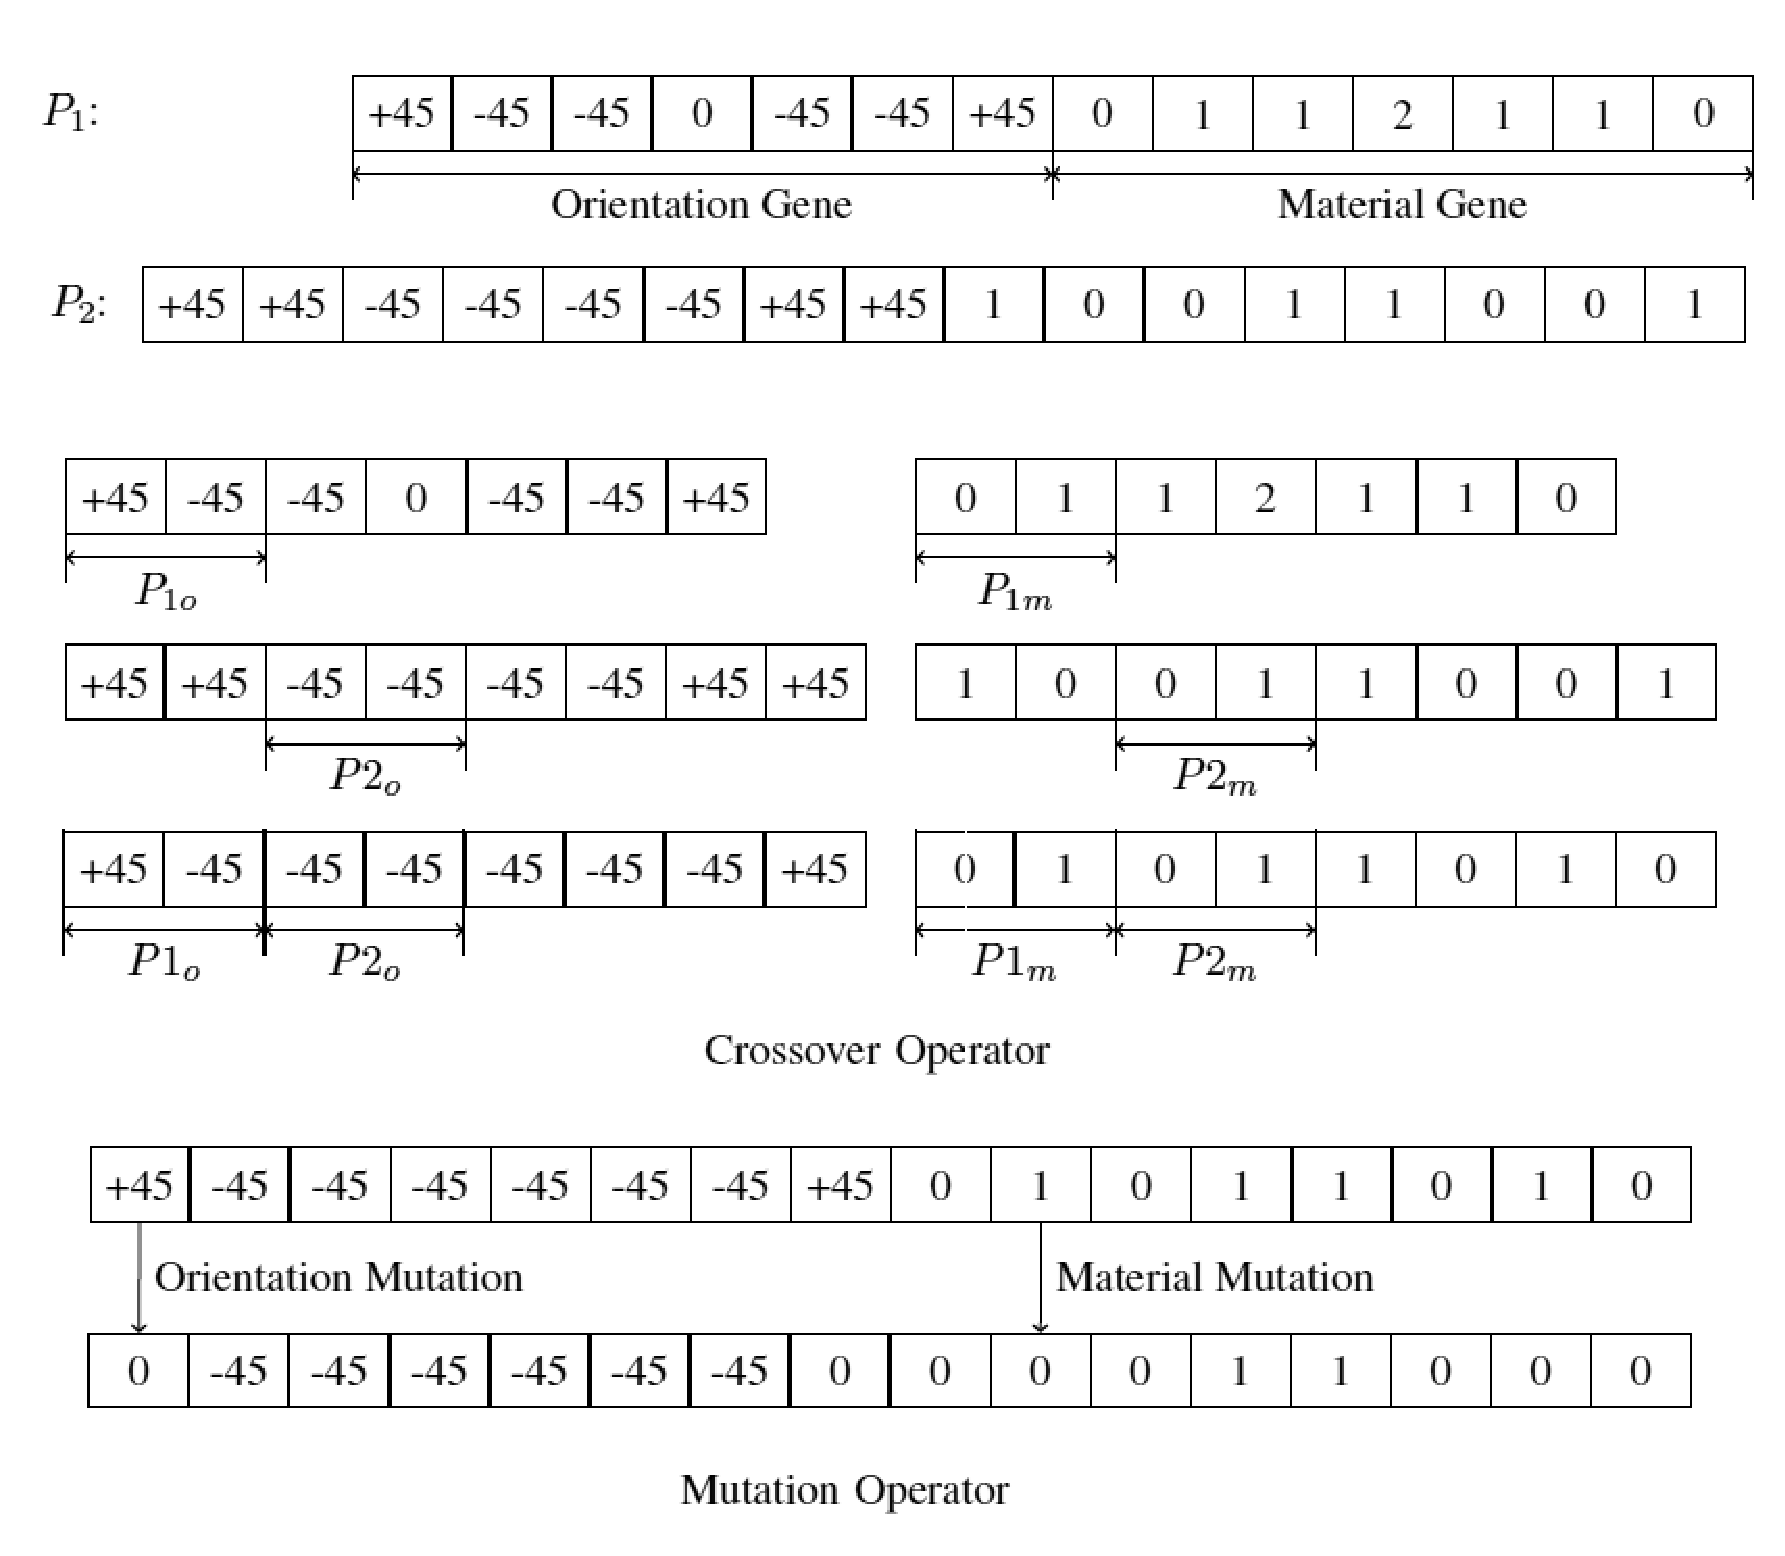
\includegraphics[width=\linewidth]{ga_operator}
%\caption{GA Operators\label{GA:operator}}
%\end{figure*}

The laminate chromosome is represented by a double-gene string that can be divided into two parts:
one part represents the angles, and the other part represents the materials (as shown in Figure
\ref{GA:operator}($P_1$)) . To maintain the diversity of the population, single-point crossover is
taken during the evolution process. The break points in the string are randomly chosen, and one of
the offspring of parent 1 (as shown in Figure \ref{GA:operator}($P_1$)) and parent 2 (as shown in
Figure \ref{GA:operator}($P_2$)) is obtained by combining the gene segments $P1_o$ and $P2_o$ and
$P1_m$ and $P2_m$, respectively. The gene code of the offspring laminate is
$[\text{+}45,\text{-}45,\text{-}45,\text{-}45,\text{-}45,\text{-}45,\text{-}45,0,1,0,1,1,0,1,0]$.


To prevent the search from becoming stuck in a local optimum, mutation is used to randomly change the
gene in the chromosome, and the offspring after the mutation operator is as shown in Figure
\ref{GA:operator}

The GA is a stochastic procedure that heavily depends on the generator of pseudorandom numbers. In
the present study, the standard Wichmann-Hill generator is used in the algorithm, which combines
three pure multiplicative congruent generators of moduli 30269, 30307 and 30323. The seed used
in this paper is 1.

\subsection{Design Problem I}

The aim is to minimize the mass of a laminate composite for a targeted strength
ratio based on the Tsai-wu failure theory. The design variable are the ply angles and the
number of layers.

Find: $\{\theta_k, n\}$ $\theta_k \in \{ 0,\text{+}45,\text{-}45,90\}$

Minimize: weight

Subject to: strength ratio and first ply failure constraint


\subsection{Design Problem II}
The aim is to minimize the weighted cost and weight of hybrid composite
laminates under various loading cases, so the design variable not only includes
the ply angles and number of layers but also the material of each lamina.


Find: $\{\theta_k,\text{mat}_k, n\}$ $\theta_k \in \{ 0,\text{+}45,\text{-}45,90\}$ $\text{mat}_k \in \{CA, GR, GL \}$

Minimize:
\begin{equation}
	F=\frac{\text { Cost }}{C_{\text {min }}}+\frac{\text { Weight }}{W_{\text {min }}}
\end{equation}

Subject to: strength ratio and first ply failure constraint


Here, CA, GF, and GL represent carbon/epoxy, graphite/epoxy, and glass/epoxy, and
$C_{\text{min}}$ and $W_{\text{min}}$ represent the cost and
weight corresponding to the laminates with a minimum cost and minimum weight
obtained from previous problem.
